\chapter{Minimalflächen\label{chapter:thema}}
\lhead{Minimalflächen}
\begin{refsection}
\chapterauthor{Nadja Rutz und Ambroise Suter}

\section{Einleitung}
\rhead{Einleitung}
Was sind Minimalflächen? 
Wie werden sie definiert? 
Warum passen sie in den Kontext dieses Buches?
Diese Fragestellungen werden im Laufe dieses Kapitel an Hand von Beispielen illustriert und erörtert.

Wie der Name erahnen lässt beschreiben Minimalflächen Flähen mit minimalem Flächeninhalt. 
Ein gängiges Beispiel aus der Physik sind Seifenfilme. Wenn die Luft auf beiden Seiten eines Seifenfilms den gleichen Druck hat, dann ist er eine Minimalfläche.


\section{Katenoid}
\rhead{Katenoid}
Wenn man zwei koaxiale Drahtringe parallel zueinander in Seifenwasser taucht, entsteht eine Rotationsfläche (Abbildung \ref{KatenoidSeifenfilm}) welche Katenoid genannt wird. 

Das Katenoid ist die erste entdeckte Minimalfläche.
Sie wurde schon 1776 von Jean Baptiste Meusnier erstmals beschrieben.
In diesem Abschnitt wird die mathematische Herleitung des Katenoids mit Hilfe der Eulerschen Differenzialgleichung der Variationsrechnung aufgezeigt.
\subsection{Beispiel Katenoid}

\begin{figure}
  \centering
  \includegraphics[scale=0.5]{minimal/Cartenoid_Foto.png}
  \caption{Seifenfilm Katenoid} 
  \label{KatenoidSeifenfilm}
\end{figure}


\begin{figure}
  \centering
  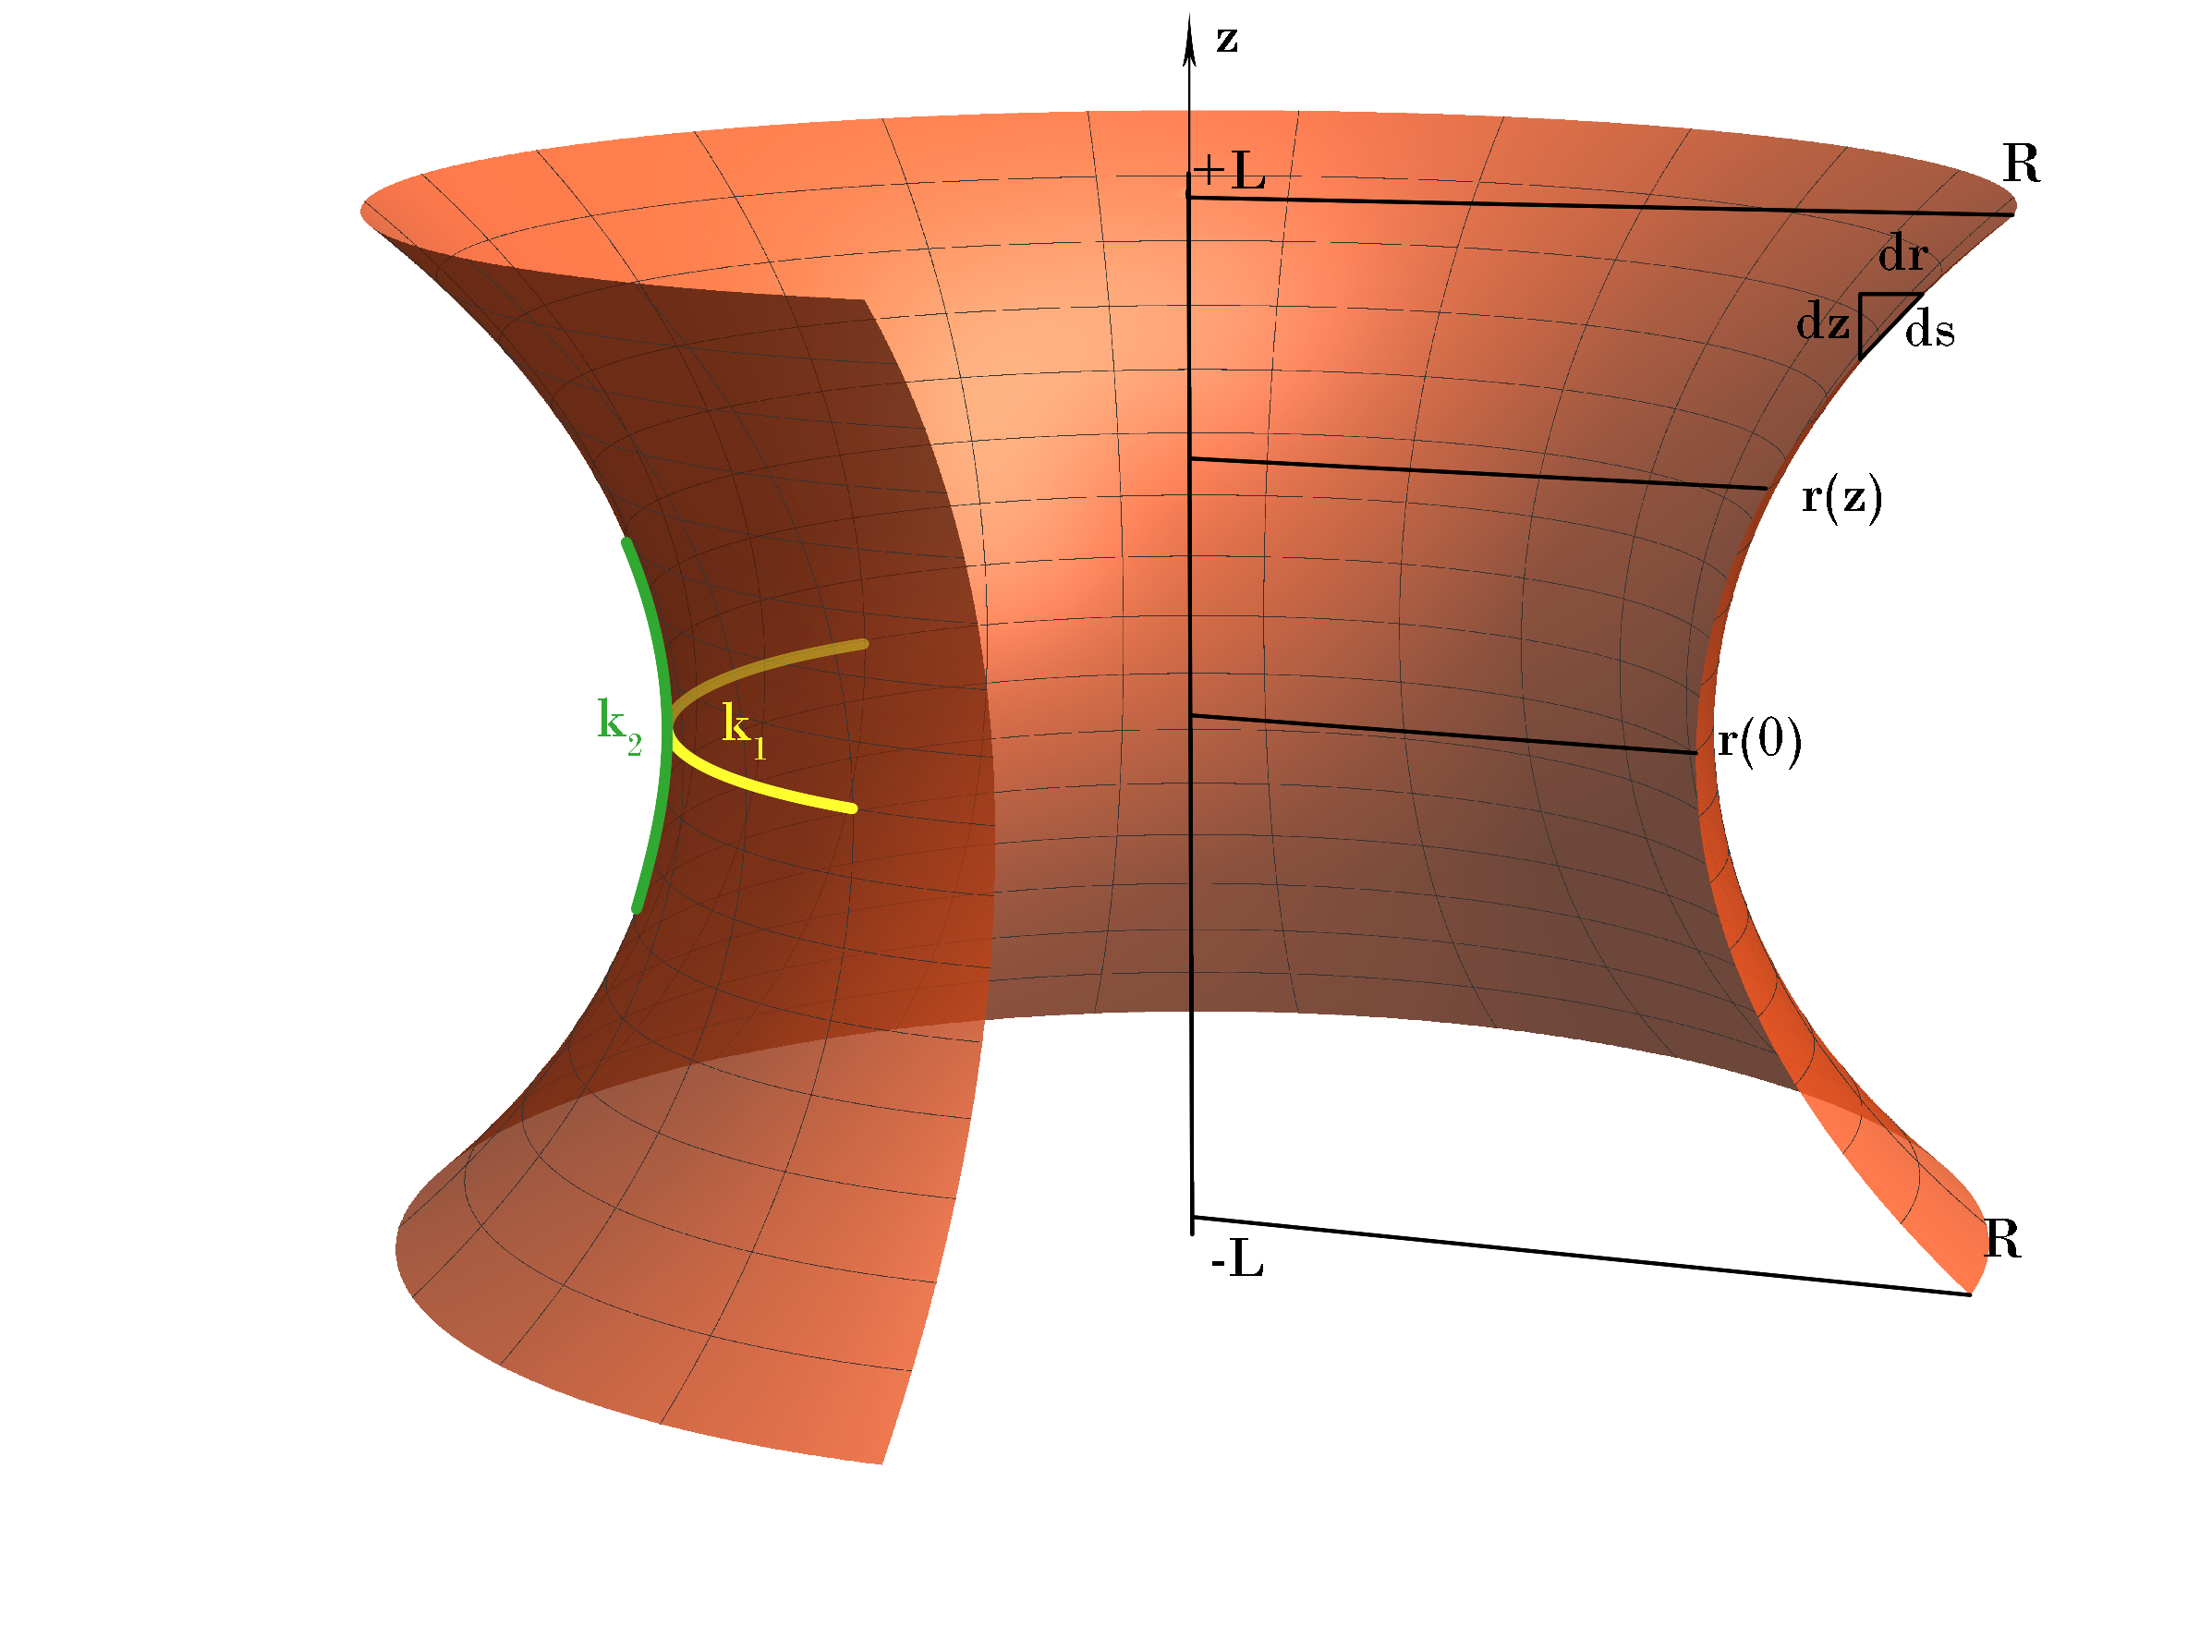
\includegraphics[scale=0.3]{minimal/Catenoid34Black.pdf}
  \caption{Skizze Katenoid} 
  \label{Katenoid}
\end{figure}
In der Skizze \ref{Katenoid} ist ein Katenoid abgebildet, bei welchem in Bezug auf die $z$ Achse, der untere Drahtring bei $-L$ und der obere bei $+L$ ist. 
Die beiden Kreise sollen die gleichen Radien haben, also gilt $r(-L)=r(+L)=R$. 
Mathematisch werden die Flächenpunkte des Katenoids mit der Funktion $r(z)$ beschrieben, diese wird um die Rotationsachse $z$ rotiert um den Flächeninhalt des Katenoids zu berechnen.
Hierzu braucht man eine Gleichung, welche eine Länge entlang eines Meridians auf der Katenoidoberfläche beschreibt. 
Mit Hilfe Satzes von Pythagoras (Abbildung \ref{Katenoid}) kann man schreiben $ds^2=dz^2+dr^2$.
Formt man diese Gleichung um, erhält man die Gleichung

\begin{equation} \label{ds}
  ds=\sqrt{dz^2\bigg(1+\frac{dr^2}{dz^2}\bigg)}= \sqrt{dz^2(1+\dot r^2)}=\sqrt{(1+\dot r^2)}\,dz .
\end{equation}
\subsubsection{Minimalfläche}
Der Seifenfilm bewegt sich automatisch in den minimalenergetischen Zustand. 
In diesem Zustand ist dann auch der Flächeninhalt $S$ des Seifenfilms minimal.
Demzufolge muss das Integral 
\begin{equation} \label{S1}  
  S= \int 2 \pi r \,ds 
\end{equation}
minimiert werden. 
Durch Einsetzen von Gleichung \eqref{ds} erhält man die Gleichung 
\begin{equation} \label{S2}
  S=2 \pi \int_{-L}^{+L} r\sqrt{1+\dot r^2}\,dz =2 \pi \int_{-L}^{+L}  F(r,\dot r, z) \,dz 
\end{equation}
welche man als Funktion 
\begin{equation} \label{F}
 F(r,\dot r, z) = r \sqrt{1+\dot r^2}
\end{equation}
noch verallgemeinert schreiben kann.



Um dieses Integral \eqref{S2} zu minimieren kann man sich der Eulerschen Differenzialgleichung der Variationsrechnung bedienen. 
\subsubsection{Variationsrechnung}
Die Eulerschen Differenzialgleichung der Variationsrechnung wird im Kapitel der  \ref{skript:geodaeten:section:variationsprinzip} Geodäten genauer erklärt.
Das Anwendungsprinzip wird hier kurz zusammengefasst. Hat man ein kompliziertes Integral, kann man die Eulersche Differentialgleichung anwenden, um die Extremwerte zu bestimmen. Diese besagt, dass anstelle des Ausrechnens  einer Integralfunktion der Art \begin{equation} \label{E_DGL1}  
  I(y)= \int_a^b F(x,y(x),\dot y(x))\,dx       
\end{equation}
kann auch die Differentialgleichung  



\begin{equation} \label{E_DGL2}
\bigg(\frac{\partial F}{\partial y}\bigg)- \frac{d}{dx} \bigg(\frac{\partial F}{\partial \dot{y}}\bigg)=0         
\end{equation}
gelöst werden, um die Extremwerte eines solchen Integrals zu finden.

Die Gleichung \eqref{S2} des Flächeninhaltes des Katenoids ist ein kompliziertes Integral, da es von der Funktion $r(z)$ abhängt und die Aufgabe ist es eben diese zu finden. Wendet man also das prinzip der Variationsrechnung an, erhält die Differentialgleichung
\begin{equation} \label{K_DGL1}
\bigg(\frac{\partial F}{\partial r}\bigg)- \frac{d}{dz} \bigg(\frac{\partial F}{\partial \dot{r}}\bigg)=0 .
\end{equation}

Setzt man F aus der Gleichung \eqref{F} ein, erhält man
\begin{equation} \label{K_DGL_H}
\sqrt{1+{\dot {r}}^2}-\frac{ d }{ dz } \bigg( r \frac{ 1 }{2  }\left( {1+{\dot {r}}^2}  \right)^{-1/2} 2 \dot {r}\bigg)=0 .
\\
\end{equation}
Dies wird nun schrittweise umgeformt zunächst durch Ausrechnen der Ableitung

\begin{equation} \label{K_DGL_H2}
\left(1+{\dot {r}}^2  \right)^{-1/2}-\bigg(r \frac{ -1 }{2  } \left({1+{\dot {r}}^2}  \right)^{-3/2} 2 \dot{r} \ddot{r}  \dot{r}+ r \left({1+{\dot {r}}^2}  \right)^{-1/2} \ddot{r} +\dot{r} \left({1+{\dot {r}}^2}  \right)^{-1/2} \dot{r}\bigg)=0
\end{equation}
bis die Differentialgleichung zweiter Ordnung  
\begin{equation} \label{K_DGL_R}
1+{\dot {r}}^2=r  \ddot{r}
\end{equation}
entsteht. 
Gesucht ist also eine Funktion $r(z)$, die die Differentialgleichung \eqref{K_DGL_R} erfüllt. Als Randbedingungen für die Funktion $r(z)$ sind in diesem Beispiel $r(+L)=R$ und $r(-L)=R$ aus der Abbildung \ref{Katenoid} gegeben.

\subsubsection{Lösen der Differentialgleichung}
Die Differenzialgleichung zweiter Ordnung \eqref{K_DGL_R} kann mit Hilfe einiger mathematischer Umformungen, Aufleiten und hyperbolischer Trigonometrie gelöst werden. 
Dies ist eine langwierige Berechnung und wird daher hier nicht durchgeführt.

Anstelle des konkreten Ausrechnens kann man die Lösung der Differentialgleichung \eqref{K_DGL_R} auch erraten. 
Aus der hyperbolischen Trigonometrie ist $\cosh^2-\sinh^2=1$ oder anders geschrieben $1+\sinh^2=\cosh^2$ \eqref{K_hTrigo} bekannt. 
Beim Ableiten von $\cosh$ erhält man $\sinh$ und $\sinh$ abgeleitet ergibt wieder $\cosh$. 
Mit dieser Erkenntnis kann man durch das Vergleichen der Gleichungen versuchen die Form der Lösung der Differentialgleichung \eqref{K_DGL_R2} zu erraten. 

Der Term $\sinh^2$  (zweiter Term links) soll der quadrierten Ableitung einer Funktion ${\dot {r}}^2$ entsprechen also kann man schreiben $(\cosh)'^2$. 
Auf der rechten Seite sollte $\cosh^2=\cosh \cosh$ dem Produkt von einer Funktion und ihrer doppelten Ableitung gleich kommen. Da gilt $(\cosh)''=(\sinh)'=\cosh$, kann die rechte Seite so $(\cosh) (\cosh)''$ auch durch $\cosh$ ausgedrückt werden.


Zusammengefasst kann man die Gleichung 
\begin{equation} \label{K_hTrigo}
1+\sinh^2=\cosh^2
\end{equation}
 in die Gleichung 
 \begin{equation} \label{K_DGL_R2}
1+{\dot {r}}^2=r  \ddot{r}
\end{equation}
 umformen und sieht mit Hilfe der Gleichung 
\begin{equation} \label{K_hTrigoU}
1+(\cosh)'^2=(\cosh) (\cosh)''
\end{equation}
dass $r(z)$ eine Funktion in $\cosh$ sein muss.
Die exakte Lösung der Differentialgleichung \eqref{K_DGL_R} beinhaltet noch die zwei Konstanten $K$ und $\xi$, welche durch die doppelte Integration dazukommen. Daraus resultiert somit für $r(z)$ die Gleichung 

\begin{equation} \label{K_r}
r(z)=K \cosh\bigg(\frac{z-\xi}{K}\bigg)
\end{equation}

Unter Einbezug der Anfangsbedingungen $r(+L)=R$ und $r(-L)=R$ aus Abbildung \ref{Katenoid} ist der Radius $R$ bei $z= \pm L$ gleich gross. Deshalb kann man $r(+L)$ mit $r(+L)$ und $R$ gleichsetzen. Durch einsetzen der Funktion $r(z)$ erhält man folglich die Gleichung
\begin{equation} \label{K_rL}
K \cosh\bigg(\frac{L-\xi}{K}\bigg)=K \cosh\bigg(\frac{-L-\xi}{K}\bigg)=R
\end{equation}

Da der $\cosh$ eine gerade Funktion ist, kommt man entweder auf $L-\xi=-L-\xi$ oder auf $L-\xi=-(-L-\xi)$. 
Beim ersten Fall wäre $L=-L$, was keinen Sinn ergibt, da dann $L=0$ wäre. Beim zweiten Fall muss $\xi=0$ sein, also muss für $K$ gelten 
\begin{equation} \label{K_rzl}
R=K \cosh\left(\frac{L}{K}\right).
\end{equation}
Die Parameter $L$ und $R$ sind vorgegeben, dass heist $K$ kann aus dieser Gleichung \eqref{K_rzl} bestimmt werden.

Daraus folgt als Lösung für das Katenoid die Funktionsgleichung 
\begin{equation} \label{K_rz}
r(z)=K \cosh\left(\frac{z}{K}\right).
\end{equation}

Noch Anzumerken ist, dass $K$ auch eine geometrische Bedeutung hat. Da $cosh(x)$ ein Minimum bei $x=0$ hat und dort den Wert $1$ annimmt, ist $K$ der minimale Wert, den $r(z)=K \cosh\left(\frac{z}{K}\right)$ annehmen kann. $K$ ist also der Radius des 
Katenoids an der engsten Stelle.

Es gibt auch einen physikalischen Grund, warum die Bestimmung des $K $ nicht ganz trivial ist. 
Stellen Sie sich vor, sie ziehen die beiden 
Drahtringe immer weiter auseinander, machen also das $L$ grösser.
Dabei wird die engste Stelle der Minimalfläche immer enger.
Irgendwann wird sie so eng, dass es für die Minimalfläche günstiger wäre, wenn sie platzen würde und stattdessen einfach jeden der Drahtringe mit einer Kreisfläche ausfüllen würde.

\section{Sattelfläche}
\rhead{Sattelfläche}
Es gibt mehrere verschiedene Arten Minimalflächen zu charakterisieren, das Beispiel des Katenoids illustriert das Konzept des minimalen Flächeninhaltes. 
Eine mathematischere charakterisierung basiert auf der sogenannten mittleren Krümmung, die in \ref{KruemmungEinerFlaeche} definiert wird.
In diesem Buch wurde bis anhin hauptsächlich die Gauss Krümmung betrachtet. 
Dies weil wir uns auf der Erde in (oder direkt auf) der zu betrachtenden Fläche befinden. 
Anders formuliert, ist die Gausskrümmung ein Mass für die innere Krümmung einer Fläche, diese Art Krümmung ist heisst intrinsische Krümmung. 
Die mittlere Krümmung im Gegensatz ist eine extrinsische Krümmung, was heisst, dass der Beobachter von aussen die Krümmung der Fläche beobachtet.
Folgend wird zuerst das Konzept der Krümmung kurz zusammengefasst und anschliessend der Unterschied der mittleren und Gauss Krümmung im Bezug auf Minimalflächen illustriert, bevor dies alles mit dem Beispiel der Sattelfläche visualisiert wird.


\subsection{Krümmung einer Fläche}
\index{Krümmung einer Fläche}
\label{KruemmungEinerFlaeche}
Intuitiv ist Krümmung einer Fläche für uns ein Mass der Abweichung der Fläche. 

Betrachtet man das Bild \ref{Kruemmungsradius} versteht man unter  dem Krümmungsradius $R$ den Radius des Kreises, welcher die Kurve in Punkt $P$ am besten approximiert. 
Da wir intuitiv bei einem Kreis oder einer Kugel eine grosse Krümmungszahl erwarten und bei einer fast ebenen Fläche eine kleine, ist die Krümmung $k$ als der Kehrwert des Krümmungsradius definiert $k=1/R$. 

Bei einer Fläche gibt es für jede Tangentenrichtung eine Kurve in der Flä-che, die diese Tangentenrichtung hat und damit auch eine Krümmung, die zu dieser Richtung gehört.
Die Extremalwerte dieser Krümmung gehören zur Tangentenrichtungen, diese stehen senkrecht aufeinander und heissen Hauptkrümmungen $k_1$ und $k_2$.

Die Tangentenrichtungen sind so definiert, dass $R_1$ den Minimalwert und $R_2$ den Maximalwert annimmt.
Die Krümmung einer Fläche im Punkt $P$ kann in der Mathematik indirekt durch die Hauptkrümmungsradien $R_1$ und $R_2$ ausgedrückt werden.


\begin{figure} 
  \centering
  \includegraphics[scale=0.1]{minimal/Kruemmungsradius.png}
  \caption{Krümmungsradius} 
  \label{Kruemmungsradius}
\end{figure}

Überträgt man das Konzept der Krümmung ins Dreidimensionale braucht es zwei Krümmungen, welche orthogonal zueinander stehen, um die Krümmung an einem Punkt zu bestimmen. Diese werden als Hauptkrümmungen $k_1$ und $k_2$ bezeichnet.
Zur nummerischen Charakterisierung der Krümmung einer Fläche in der Mathematik werden hauptsächlich zwei Grössen benutzt.
Zum einen die Gauss Krümmung, welche eine intrinsische Krümmung ist und zum andern die mittlere Krümmung bei welcher es sich um eine extrinsische Krümmung handelt. Bei Minimalflächen ist vor allem die mittlere Krümmung von Bedeutung.


\index{Gauss Krümmung}
\subsubsection{Gauss Krümmung}
Die Gauss Krümmung einer Fläche im Punkt $P$ ist definiert als das Produkt der zwei Hauptkrümmungen $k_1$ und $k_2$.

\begin{equation} \label{Gauss_Kruemmung_D}
  H=k_1\, k_2= \frac{1}{R_1}\frac{1}{R_2}
\end{equation}



Die Gauss Krümmung ist eine intrinsische Krümmung. Ein Mass für die innere Krümmung der Fläche. 

Eine gute Vorstellungshilfe ist die Ameisenperspektive. 
Wenn die Ameise auf einer Kugel ist kann sie feststellen, dass nur schon in ihrem kleinen Blickfeld die Winkelsummen eines Dreiecks auf der Oberfläche grösser als 180° ist, demzufolge besitzt die Kugel eine positive Gauss Krümmung. Anders sieht es aus bei einem Zylinder dort misst die Ameise auf der Zylinderoberfläche genau 180° Winkelsumme, dass heisst die Gauss Krümmung eines Zylinders ist null. 

Im Kontext dieses Buches ist noch zu erwähnen, dass für Flächen die Gauss Krümmung ge-nau dem Krümmungsskalar entspricht, dieses wurde im früheren Verlauf des Buches aus dem Riemann-Tensor abgeleitet (\ref{skript:maxima:curvature}).

\index{mittlere Krümmung}
\subsubsection{Mittlere Krümmung}
Die mittlere Krümmung einer Fläche im Punkt $P$ ist definiert durch den Mittelwert der zwei Hauptkrümmungen $k_1$ und $k_2$.

\begin{equation} \label{Mittlere Kruemmung_D}
  H=\frac{1}{2}(k_1+k_2)= \frac{1}{2}\bigg(\frac{1}{R_1}+\frac{1}{R_2}\bigg)
\end{equation}

Die mittlere Krümmung ist eine extrinsische Krümmung. 
Im Gegensatz zur intrinsischen Krümmung kommt es bei einer extrinsischen Krümmung auf die Umgebung an. 
Man kann sich vorstellen, dass man zum Beispiel die Krümmung eines Zylinders (zweidimensionales Objekt) von aussen, also in einem dreidimensionalen Raum betrachtet. 
Ein Zylinder ist aus der Ameisenperspektive flach, schaut man von aussen, sieht er jedoch gekrümmt aus.
Dies, weil er eine positive mittlere Krümmung aufweist. 
Anders sieht es zum Beispiel bei einer Sattelfläche (Pringels-Chips artigen Fläche) aus, dort ist die Gausskrümmung negativ, hingegen kann die mittlere Krümmung im Spezialfall, dass $R_1=-R_2$, also die Krümmungsradien ein umgekehrtes Vorzeichen aufweisen, aber vom Betrag her identisch sind, gleich null sein. 
In diesem Fall ist diese Sattelfläche ein Beispiel für eine Minimalfläche.
Die besondere Bedeutung der mittleren Krümmung H besteht darin, dass Minimalflächen dadurch charakterisiert sind, dass für sie gilt $H=0$. Diese Eigenschaft führt auch dazu, dass jeder, genügend kleine Ausschnitt einer beliebigen Minimalfläche eine Sattelfläche ist. Nimmt man beispielsweise das Katenoid und halbiert es senkrecht erkennt man die vorhandene Sattelfläche.

Im Abschnitt \ref{Young-Laplace} wird die Young-Laplace-Gleichung hergeleitet, welche erklärt warum Minimalflächen die Eigenschaft $H=0$ haben muss, beziehungsweise was $H \neq 0$ bedeutet.  

\begin{figure} 
  \centering
  \includegraphics[scale=0.4]{minimal/Tabelle_Kruemmung.png}
  \caption{Vergleich Grauss und Mittlerekrümmung} 
\end{figure}




\subsection{Beispiel Scherksche Sattelfläche}
\begin{figure}
  \centering
  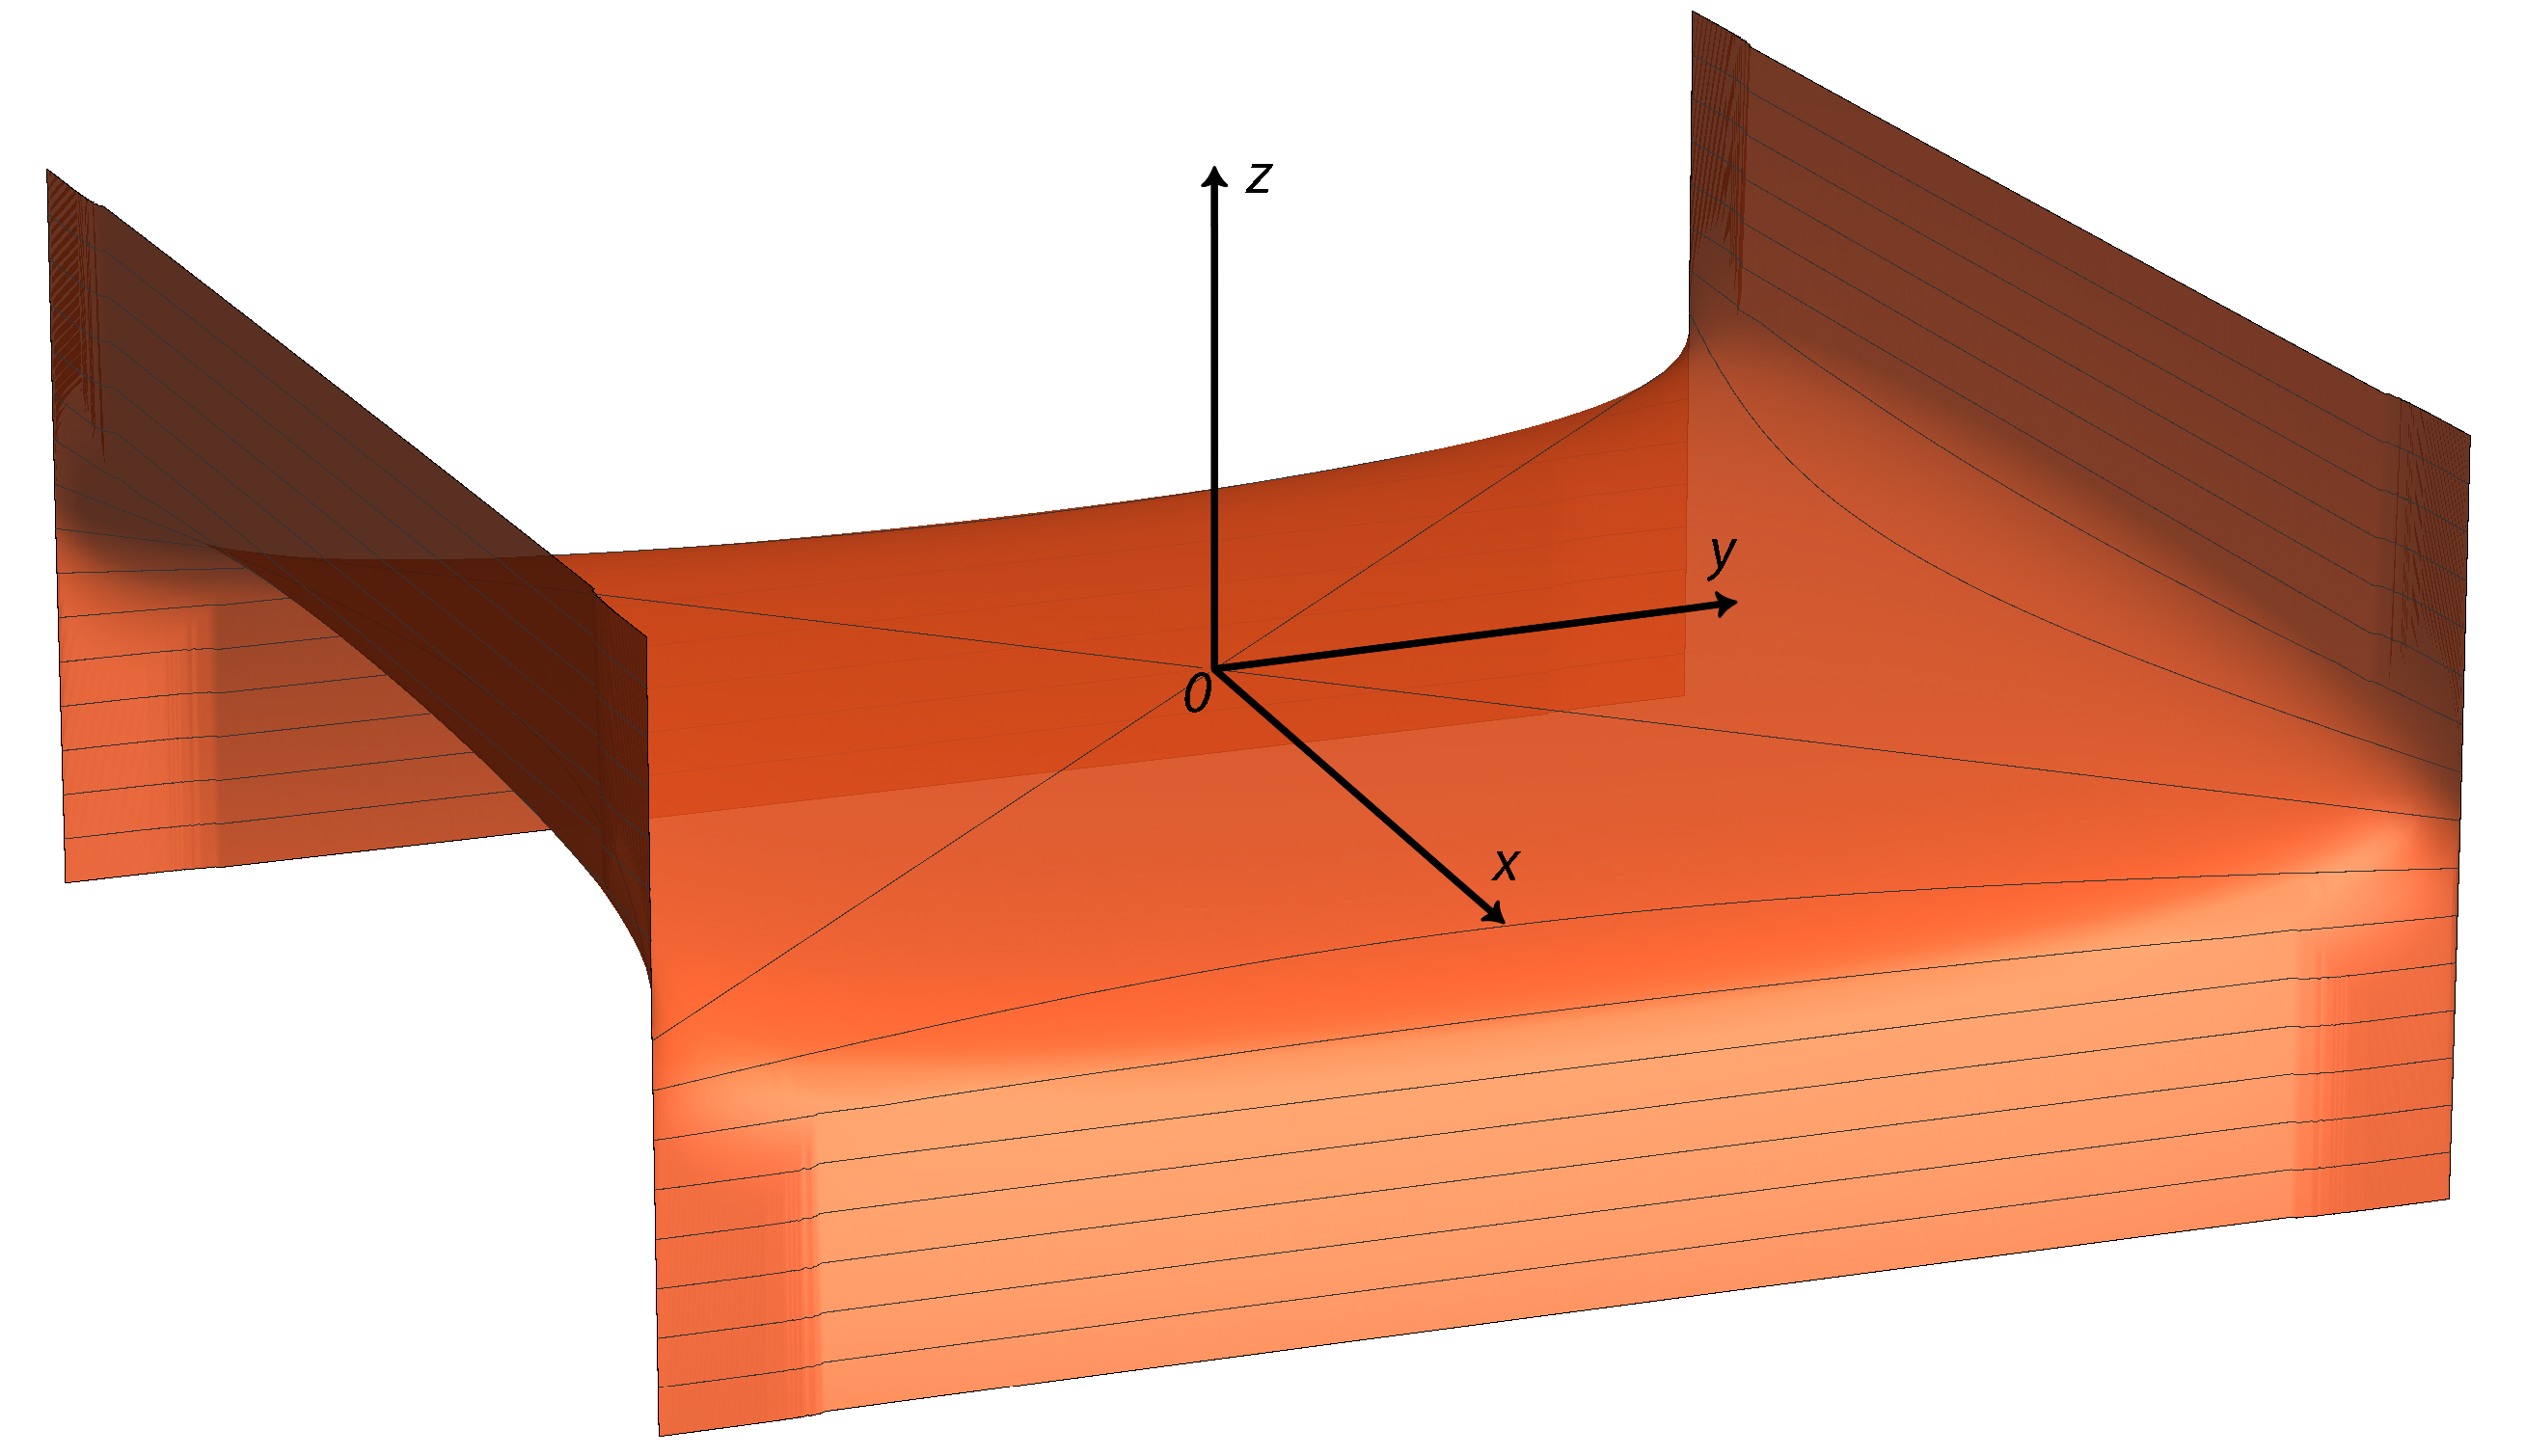
\includegraphics[scale=0.3]{minimal/HFSherckV2.pdf}
  \caption{Sattelfläche von Scherk} 
  \label{fig:Scherk}
\end{figure}
Die Scherksche Sattelfläche \. (Abbildung: \ref{fig:Scherk})\, hat neben den zwingenden Eigenschaften einer Minimalfläche, deren Gausskrümmung kleiner als null ist und die zusätzlich eine mittlere Krümmung von genau null hat, die Eigenschaft, dass sie, im Gegensatz zur Rotationsfläche des Katenoids, der Graph einer Funktion $z=Z(x,y)$ ist. Sie ist neben der trivialen Ebene eine der wenigen Minimalflächen mit dieser Eigenschaft.

Eine Approximation an die Fläche kann mittels Drahtgeflecht und einer Seifenlösung nachgebildet werden \. (Abbildung: \ref{fig:SoapScherk}). Die einzelnen Seifenmoleküle versuchen ein stabiles Gleichgewicht der abstossenden und anziehenden Kräfte zu finden. Dieser stabile Punkt braucht durch das Gleichgewicht ein Minimum an Energie. Dies bedeutet auch, dass die Krümmung, welche Energie benötigt, minimiert wird.
\begin{figure}
  \centering
  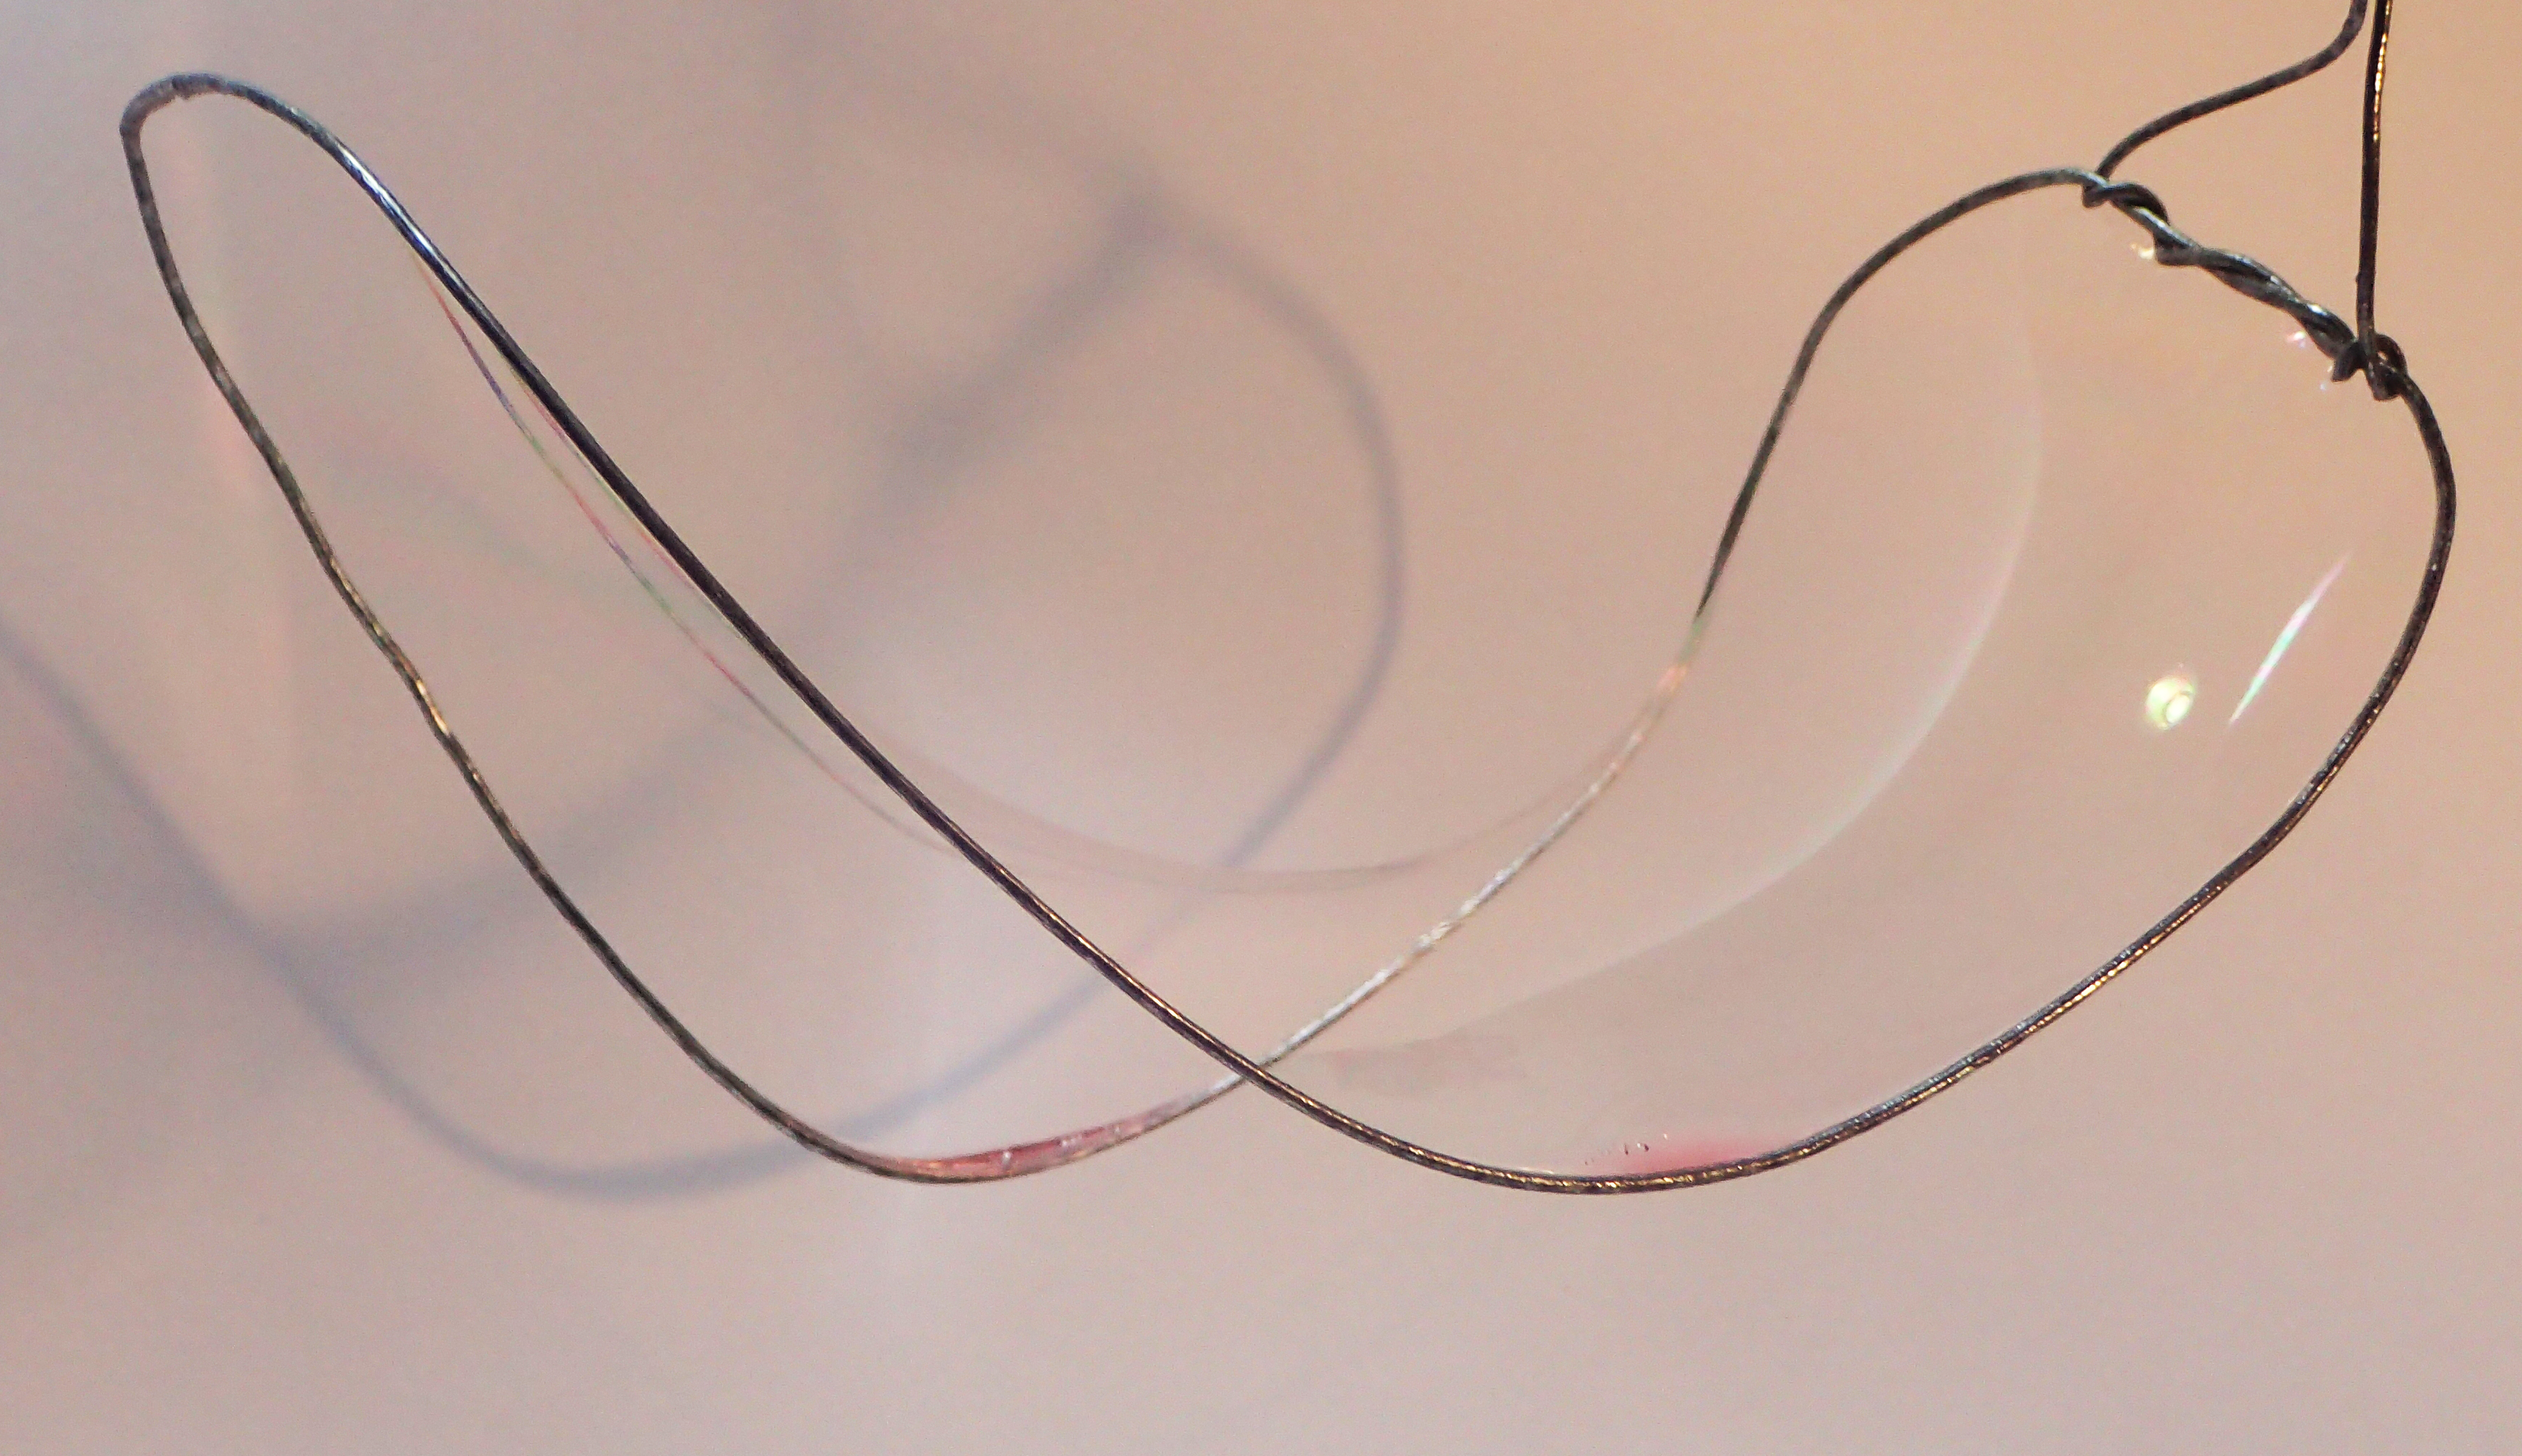
\includegraphics[scale=0.4]{minimal/SattelflacheSoapFilm.png}
  \caption{Seifenfilm bildet Minimalfläche} 
  \label{fig:SoapScherk}
\end{figure}
Die Sattelfläche wurde erstmals 1834 von Prof. H. F. Scherk beschrieben cite{minimal:JournalAM} und hergeleitet. Sie war nach der in 1776 von Meusnier beschriebene Katanoid die erste neue Minimalfläche. 

Die noch unbekannte Funktion $z=Z(x,y)$ um die Minimalfläche zu beschreiben wird mit mittels Minimalflächengleichung (im Englischen unter dem Namen Minimal Surface Equation bekannt) cite{minimal:Osserman}
\begin{equation}\label{MFG}
(1+ Z_x^{2})Z_{xx} - 2 Z_x Z_y Z_{xy} + (1+ Z_x^{2}) Z_{yy}=0
\end{equation}
berechnet. 

Die Minimalflächengleichung ist eine partielle Differentialgleichung welche durch Lösen der Euler-Lagrange Gleichung \ref{skript:geodaeten:subsection:Euler-Lagrange-Gleichung} für Flächen mit mittlerer Krümmung $H=0$ gefunden wird. Das Lösen derselben würde den Rahmen hier aber deutlich übersteigen. 

$Z_x$ ist die erste Ableitung der Funktion $Z(x,y)$ nach $x$. $Z_y$ ist analog dazu die erste Ableitung der Funktion $Z(x,y)$ nach $y$. $Z_{xx}$ und $Z_{yy}$ sind die jeweils 2. Ableitungen der Funktion $Z(x,y)$ nach den entsprechenden Indizes. $Z_{xy}$ ist die Ableitung von $Z_x$ nach $y$. Beziehungsweise die Funktion $Z(x,y)$ erst nach $x$ und dann zusätzlich nach $y$ abgeleitet. 

Zusätzlich stellen wir zwei Nebenbedingungen. Die erste Bedingung, $Z(0,0)=0$, bedingt, dass der Graph im Nullpunkt auf der Höhe null ist. Die zweite, $\nabla Z(0,0)=0$, fordert, dass im Nullpunkt der Graph in alle Richtungen flach ist.

\subsubsection{Lösen der Partiellen Differentialgleichung}\label{Scherk Berechnung}
Angenommen $z=Z(x,y)$ ist der Graph einer Funktion. Wobei ${x,y}$ die Koordinaten in der Ebene sind, welche nach $z$ Abgebildet werden (siehe Abbildung \ref{fig:Scherk}). 

Um die Minimalflächengleichung zu lösen nehmen wir an, dass die Funktion $Z(x,y)$ eine lineare Zusammensetzung von zwei Funktionen ist. Die einfachste Möglichkeit dies zu erreichen, ist die Addition von zwei Funktionen: $z=Z(x,y)=f(x)+g(y)$. Dieser glückliche Ansatz ist nur eine von vielen Möglichkeiten eine partielle Differentialgleichung zu lösen. 

Wir setzen die benötigten Ableitungen und mehrfachen Ableitungen der Funktion $Z(x,y)$ in die Minimalflächengleichung (\ref{MFG}) ein. Da $ Z_x = f'(x),\ Z_y = g'(y),\ Z_{xx}=f''(x),\ Z_{yy} = g''(y) \ \text{und} \ Z_{xy}=0$ ist, vereinfacht sich die Minimalflächengleichung zu 
\begin{equation}\label{MFG Scherk}
(1+g'(y)^2)f''(x)+(1+f'(x)^2)g''(y)=0
\end{equation}
Durch Separieren von $f$ und $g$ erhalten wir zwei gewöhnliche Differentialgleichungen 2. Ordnung
\begin{equation}\label{MFG Scherk2}
-\dfrac{f''(x)}{1+(f'(x))^2}=\dfrac{g''(y)}{1+(g'(y))^2}=c
\end{equation}
mit $c \in \mathbb{R}$ konstant. $c$ ist Konstant, da die Gleichung nur stimmen kann, wenn trotz unterschiedlichen Variablen $x$ und $y$ beide Quotienten bei einer Veränderung in $x$- beziehungsweise $y$-Richtung gleich bleiben. Wird zum Beispiel $x=0$ fixiert und $y$ variiert muss die Differentialgleichung in $g(y)$ konstant bleiben, da sonst die Gleichung durch die Veränderung des 2. Quotienten ungleich wäre.

Die Differenzialgleichungen in $f$ und $g$ werden nun separat gelöst. Erst wird $f'(x)$ mit $w(x)$ substituiert. 
\begin{equation}\label{ScherkDGL1}
-\dfrac{w'(x)}{1+w(x)^2}= c  , \quad w(x)=f'(x).
\end{equation}
Anschliessend wird die Gleichung  beidseitig integriert
\begin{equation}
\int -\dfrac{w'(x)}{1+w(x)^2} dx = \int c \ dx
\end{equation}
und wir erhalten die folgende Gleichung:
\begin{equation}
-\arctan(w(x)) = cx+k_1
\end{equation}
welche wir nach $w(x)$ auflösen.
\begin{equation}
w(x) = -\tan(cx+k_1).
\end{equation}
Wir führen eine Rücksubstitution durch und erhalten
\begin{equation}\label{SchreckDGL2}
f'(x) = -\tan(cx+k_1).
\end{equation}
Um die Lösung der Differentialgleichung zu erhalten Integrieren wir erneut
\begin{equation}
\int f'(x)\ dx = \int -\tan(cx+k_1)\ dx.
\end{equation}
 Die Lösung lautet gemäss Integrationstabelle
\begin{equation}
f(x) = \dfrac{\log(\cos(cx+k_1))}{c}+k_2.
\end{equation}
Mit den Nebenbedingung $f(0)=0$ und $f'(0)=0$ ergibt sich $k_1=k_2=0$ und wir erhalten die gesuchte Gleichung 
\begin{equation}
f(x) = \dfrac{\log(\cos(cx))}{c}.
\end{equation}
Analog dazu ergibt sich für die 2. Differenzialgleichung:
\begin{equation}
g(y) = - \dfrac{\log(\cos(cx))}{c}.
\end{equation}
Somit lautet die Funktion $Z(x,y)$ der Scherkschen Minimalfläche
\begin{equation}
Z(x,y)=\dfrac{\log(\cos(cx))}{c}-\dfrac{\log(\cos(cy))}{c}.
\end{equation}

\subsection{Beispiel Young–Laplace - Oberflächenspannung}
\rhead{Young–Laplace}
\label{Young-Laplace}

\label{YL-Beschreibung}
In den vorangegangenen Beispielen wurde jeweils eine Lösung gesucht, bei der die Mittlere Krümmung $H=0$ ist. Bei den meisten Oberflächen ist dies jedoch nicht der Fall. Beispielsweise haben Seifenblasen innen und aussen einen anderen Druck. Oder in einem Blutgefäss herrscht innen der Blutdruck und außerhalb der Druck durch die Gewebe. Diese Druckdifferenz wirkt eine Kraft auf eine Oberfläche ein und verunmöglicht damit eine minimale Oberfläche wie bei einer Minimalfläche.

Dennoch haben solche Oberflächen ähnliche Eigenschaften, da auch hier die Energie minimiert wird. Dies wird durch die Young-Laplace Gleichung \cite{minimal:Laplace} beschrieben, welche im folgenden Abschnitt mittels geometrischen und physikalischen Überlegungen hergeleitet wird.
\subsubsection{Herleitung der Young-Laplace Gleichung}\label{YL-Herleitung}
Angenommen zwei Medien (z.B. Luft/Wasser) werden durch eine Oberfläche \, (Abbildung: \ref{fig:YoungCone}) getrennt. Da in den Medien verschiedene Drücke $p_1$ und $p_2$ herrschen, wölbt sich die Oberfläche. Die Veränderung des Krümmungsradius sei $\delta\zeta$ \,(Abbildung: \ref{fig:Strahlensatz}). Das Volumen eines einzelnen infinitesimalen Volumensegments sei $\delta\zeta\,dA$ \,(Abbildung: \ref{fig:Volumentransaltion}). Dann ist die benötigte Arbeit um das Volumensegment um $\delta\zeta$ zu verschieben:
\begin{figure}
  \centering
  \includegraphics[scale=0.3]{minimal/YoungCone.png}
  \caption{Ausschnitt aus einer Oberfläche mit Krümmungsradien} 
  \label{fig:YoungCone}
\end{figure}
\begin{figure}
  \centering
  \includegraphics[scale=0.3]{minimal/Volumetranslation.png}
  \caption{Element der Volumentranslation} 
  \label{fig:Volumentransaltion}
\end{figure}
\begin{equation}
\delta W=\int(-p_1+p_2)\,\delta\zeta\,dA.
\end{equation}
Die Gesamte Arbeit ergibt sich, wenn zur Arbeit der Volumenänderung die Arbeit der Veränderung der Oberfläche $\delta W=\gamma \, \delta A $ dazu addiert wird, wobei $\gamma$ die Oberflächenspannung und $\delta A$ die veränderte Oberfläche ist. Wir erhalten
\begin{equation}\label{YL-Arbeit_1}
\delta W=\int(-p_1+p_2)\,\delta\zeta dA + \gamma \,\delta A.
\end{equation}
Sind $R_1$ und $R_2$ die Krümmungsradien der Oberfläche, werden die infinitesimalen Längenstücke $dl_1$ und $dl_2$ bei einer Veränderung der Radien $R$ um $\delta\zeta$ mittels Strahlensatz \.(Abbildung: \ref{fig:Strahlensatz})
\begin{equation}
\frac{R}{dl}=\frac{R+\delta\zeta}{dl+x}
\end{equation}
verlängert. Wobei $dl+x=dl'$ ist. Nach $dl'$ aufgelöst ergibt sich
\begin{equation}
dl' = dl(\frac{R+\delta\zeta}{R})
\end{equation}
durch einfache Umformungen erhalten wir
\begin{equation}
\begin{split}
dl' &= dl(1+\frac{\delta\zeta}{R})\\
&=dl+\frac{dl\,\delta\zeta}{R}
\end{split}
\end{equation}
\begin{figure}
  \centering
  \includegraphics[scale=0.3]{minimal/Langenanderung.png}
  \caption{Längenänderung} 
  \label{fig:Strahlensatz}
\end{figure}
Das Flächenstück $dA=dl_1 dl_2$ verändert sich somit
\begin{equation}
\begin{split}
dA' &= (1+\frac{\delta\zeta}{R_1})\, dl_1 (1+\frac{\delta\zeta}{R_2}) \, dl_2 \\
&\approx dl_1\,dl_2\,(1+\frac{\delta\zeta}{R_1} + \frac{\delta\zeta}{R_2}).
\end{split}
\end{equation} 
Somit ist die Änderung eines Flächenstück $\delta dA=dA'-dA$
\begin{equation}
\begin{split}
\delta dA &= dl_1\,dl_2\,\delta\zeta\,(1+\frac{1}{R_1}+\frac{1}{R_2})-dl_1\,dl_2\\
&= dl_1\,dl_2\,\delta\zeta\,(\frac{1}{R_1}+\frac{1}{R_2}).
\end{split}
\end{equation}
Um die gesamte veränderte Oberfläche zu erhalten, Integrieren wir die Änderung der Flächenstücke über die gesamte Oberfläche
\begin{equation}
\delta A = \int \delta\zeta \, \bigg( \frac{1}{R_1}+\frac{1}{R_2} \bigg)\,dA.
\end{equation}
Die veränderte Oberfläche setzen wir in die Gleichung der Variation der Arbeit \ref{YL-Arbeit_1} ein. 
Befindet sich die Oberfläche im Gleichgewicht, muss auch die Variation der Arbeit gleich Null sein.
\begin{equation}
\delta W = \int \delta\zeta \, \bigg[ (-p_1+p_2)-\gamma \, \bigg( \frac{1}{R_1}+\frac{1}{R_2} \bigg) \bigg]\,dA =0.
\end{equation}
Da $\delta\zeta=0$ eine triviale Lösung wäre, ist $\delta\zeta \neq 0$. Daraus folgt die Young-Laplace Gleichung:
\begin{equation}
-p_1+p_2 = \gamma \, \bigg( \frac{1}{R_1}+\frac{1}{R_2} \bigg)
\end{equation}
oder
\begin{equation}\label{Young-Laplace}
\Delta p = \gamma \, \bigg( \frac{1}{R_1}+\frac{1}{R_2} \bigg).
\end{equation}
Anzumerken ist, dass sie der Gleichung der mittleren Krümmung (\ref{Mittlere Kruemmung_D}) bis auf $2\gamma$ entspricht. Wir lösen die Gleichung der mittleren Krümmung nach $\bigg( \frac{1}{R_1}+\frac{1}{R_2} \bigg)$ auf und erhalten
\begin{equation}
\bigg( \frac{1}{R_1}+\frac{1}{R_2} \bigg)=2H.
\end{equation}
Somit kann man die Young-Laplace Gleichung auch als
\begin{equation}\label{YL-Result2}
\Delta p=2\gamma H
\end{equation}
schreiben.

\subsection{Anwendung: Druck innerhalb eines Regentropfens}
Nehmen wir an, ein Regentropfen wird nicht durch den Luftwiederstand verformt so bildet er eine Kugel. Da bei einer Kugel $R_1=R_2=r$ gilt, vereinfacht sich die Young-Laplace Gleichung \ref{Young-Laplace} zu
\begin{equation}
\Delta p = 2\gamma \, \bigg(\frac{1}{r}\bigg).
\end{equation}
Bei einem Radius von $0.2mm$ und einer Oberflächenspannung von $72.75 mN/m$ erhalten wir eine Druckdifferenz von
\begin{equation}
\Delta p = 2*72.75 mN/m \, \bigg(\frac{1}{0.2mm}\bigg)= 727.5 Pa,
\end{equation}
was in der Grössenordnung von einem Hundertstel des atmosphärischen Drucks liegt. 

\subsection{Anwendung: Seifenblasen sind keine Minimalfläche}
Mithilfe der bei \ref{YL-Result2} gewonnen Erkenntnis können wir leicht erkennen, dass bei einem Druckunterschied auf beiden Seiten eines Seifenfilms, Beispielsweise bei einer Seifenblase, die mittlere Krümmung nicht null sein kann. Somit kann eine Seifenblase nicht eine Minimalfläche sein.


\printbibliography[heading=subbibliography]
\end{refsection}
